\chapter{Conclusion}
\label{sec:conclusion}
\setstretch{\lspac}

In the thesis we deal with various improvements that make permutation tests more widely applicable, and show an example of such use for the analysis of cortical anatomy of the cerebrum.

Chapter~\ref{sec:ptree} shows that the multi-level block permutation effectively controls the false positive rate, even in the presence of strong dependence between observations, and can be used as a general inference tool when the dependence structure can be organised in blocks, hierarchically if necessary. There is an unavoidable loss of power due to the reduced scope of shuffling, although in large datasets, even if with relatively complex dependence structure, such as the \textsc{hcp}, this loss is expected to be quite small, especially if permutations can be combined with sign flippings.

Chapter~\ref{sec:accel} shows that a number of statistical devices can be considered to accelerate permutation tests in addition to, or irrespective of, generic improvements to accelerations that depend on software implementation or on hardware. The methods considered yielded generally similar results, and as the different scenarios of error terms and shuffling strategy varied, the methods performed only marginally better or worse than each other in terms of conservativeness, agreement with the reference set, and resampling risk, and were in general substantially faster than the alternative of running a large number of permutations.

Chapter~\ref{sec:cortex} shows that a joint analysis of cortical thickness and cortical surface area can reveal patterns of cortical pathology that would remain unseen with the usual methods that measure cortical volume. It also introduces a geometrically exact method to measure such volume, and provides a much needed comparison between the four extant methods to resample cortical area and related measurements that require mass conservation.

The hope is that these methods will help to accelerate the pace in which discoveries are made, while maintaining the hallmarks of permutation tests: robustness, exactness, and strong control over error rates.

\section{Applications and future work}

The thesis opens new avenues for research. In particular, permutation tests for large datasets, that could not be considered due to the elevated computational load, should become feasible with the acceleration strategies proposed in Chapter~\ref{sec:accel}, which can be further combined with general software and hardware improvements. Moreover, the fact that some of the acceleration methods, such as tail approximation, gamma approximation, and the no permutation, allow continuous p-values to be found, tends to increase the power of methods for corretion for multiple testing, such as false discovery rate \citep[\textsc{fdr};][]{Genovese2002}, and can be considered in tandem with the \textsc{npc}, so as to produce continuous p-values for partial tests before their combination. Investigation into these topics can be considered for future work.

The multi-level block permutation discussed in Chapter~\ref{sec:ptree} is currently the only method that can yield valid inferences for data from the Human Connectome Project, and has been used, for instance to identify a mode of population covariation that links various imaging and non-imaging variables \citep{Smith2015}.

The joint analysis introduced in Chapter~\ref{sec:cortex} is expected to provide a more informative option over the analysis of cortical volume. The method can be used to study pathological conditions affecting the cortex, but also, to provide localising power for such effects. Moreover, in being mass-con\-ser\-va\-ti\-ve, it has potential to help, for instance, to elucidate general questions, such as those related to the recent debate on whether regional proportions within the neocortex would be relatively constant across primates \citep{Schoenemann2005, Barton2013, Gabi2016}. 

In addition to the above, future work that can be considered immediately after the thesis consists of using both the multi-level block permutation and the acceleration strategies to allow faster, exact, multi-level inference for \textsc{fmri} data \citep{Woolrich2004}, in a frequentist manner, yet free from assumptions related to frequency distributions. Such inference could replace current mixed-effects strategies that are based on parametric tests, or purely fixed or random-effects currently possible with permutation, yet without permuting \textsc{fmri} time series. The acceleration strategies can likewise be considered for other cases of non-parametric combination that can be computationally onerous, such as for the statistical treatment of designs with missing data, especially when such missingness is not at random, which requires joint modelling of a potentially large number of designs.

\section{Availability}
\label{sec:conclusion:palm}

A working implementation for Octave/\textsc{matlab} of all the permutation methods presented in this thesis are available under the General Public Licence (\textsc{gpl}) in the tool \emph{Permutation Analysis of Linear Models} (\textsc{palm}), which can be downloaded freely from \href{http://www.fmrib.ox.ac.uk/fsl}{www.fmrib.ox.ac.uk/fsl}. Additionally, \textsc{palm} includes various other features that were not discussed in the thesis, and which were presented elsewhere.

%\begin{figure}[tp]
%\begin{center}
%\centerline{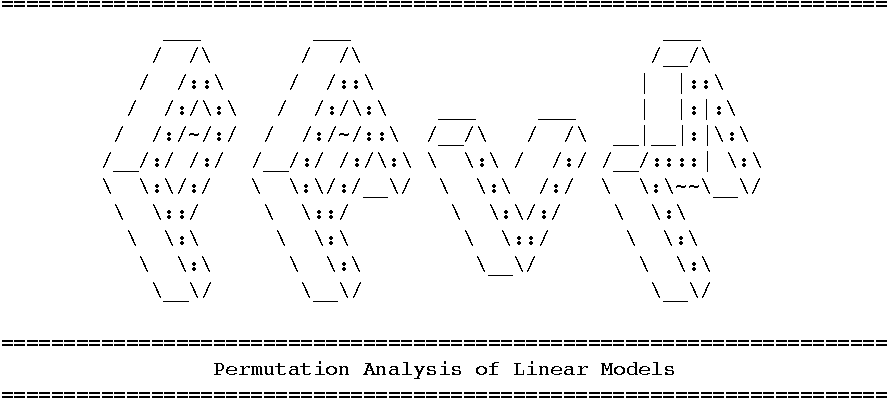
\includegraphics[width=12cm]{figures/palm-logo.pdf}}
%\end{center}
%\caption[Screen shot of \textsc{palm}.]{The methods presented in Chapters \ref{sec:ptree} and \ref{sec:accel} are available in the tool \emph{Permutation Analysis of Linear Models} (\textsc{palm}), a text-based application that can be invoked from scripts.}
%\label{fig:concl:palm-logo}
%\end{figure}

